\chapter{OVOS Implementation}
\label{ch:method}

In this chapter we build on the theoretical foundation laid out in Chapter~\ref{ch:theory} to describe the practical implementation of the OVOS algorithm. The implementation was written up for this project in Python. The goal is to provide a clear and detailed overview of the algorithmic steps, the computational strategies employed, and the choices made in the implementation, for the full implementation details see Appendix~\ref{appc:code}. 
This chapter serves as a bridge between the abstract theoretical concepts and the concrete computational details, enabling readers to understand how the OVOS method is realised and how it can be reproduced or extended in future work. It is to be made clear here that the OVOS algorithm was coded up from scratch by myself, following the original proposal by Adamowicz \& Bartlett, but with some modifications and optimisations as described in the sections below.


\section{Algorithm}
\label{sec:method_algorithm}

Here we outline the full OVOS algorithm as implemented in this work, following the general structure proposed by Adamowicz \& Bartlett \cite{Adamowicz1987}. The algorithm consists of an initialisation phase followed by an iterative loop that optimises the active virtual orbitals to maximise the MP2 correlation energy. The key steps are summarised as pseudocode in Algorithm~\ref{alg:ovos}, which serves as a roadmap for the detailed descriptions in the subsequent sections.

\begin{algorithm}[H]
\caption{OVOS Iterative Optimisation}
\label{alg:ovos}
\begin{algorithmic}[1]
  \State Perform SCF calculation to obtain initial MO coefficients $\mathbf{C}$
  \State Transform AO integrals to MO basis: $\langle ij|ab\rangle$
  \State Select initial active virtual space
  \Repeat
    \State Compute MP1 amplitudes $t_{ij}^{ab}$ and MP2 energy $J_2$
    \State Assemble gradient $\mathbf{G}$ and Hessian $\mathbf{H}$
    \State Solve Newton-Raphson equation: $\Delta\mathbf{R} = -\mathbf{H}^{-1}\mathbf{G}$
    \State Generate unitary matrix $\mathbf{U} = \exp(\mathbf{R})$
    \State Update MO coefficients: $\mathbf{C} \leftarrow \mathbf{C}\,\mathbf{U}$
    \State Canonicalise active Fock block
    \State Evaluate new $J_2$
  \Until{$|J_2^{(n)} - J_2^{(n-1)}| < \epsilon_{\mathrm{conv}}$}
\end{algorithmic}
\end{algorithm}

Below we provide a detailed description of each step in the algorithm.
\newpage

\subsection{Integral Transformation}

Transforming the two-electron integrals from the atomic orbital (AO) basis to the molecular orbital (MO) basis is a critical step in the OVOS algorithm. This transformation is necessary to compute the MP1 amplitudes and the gradient of the MP2 energy with respect to orbital rotations. However, performing a full 4-index transformation of all integrals would be computationally prohibitive. To mitigate this, we only transform the subset of integrals that are required for the MP2 amplitude equations, specifically those of the form $\langle ij|ab\rangle$ where $i,j$ are occupied orbitals and $a,b$ are active virtual orbitals, as these are the only ones that contribute directly to the correlation energy and its gradient. The transformation is performed using the \texttt{ao2mo.kernel()} function from the PySCF library, which efficiently computes the required blocks of integrals. After obtaining the spatial integral blocks for $\alpha\alpha$, $\beta\beta$, and $\alpha\beta$ spin combinations, we construct the full spin-orbital ERI tensor by interleaving the $\alpha$ and $\beta$ contributions according to the index mapping. Finally, we convert the chemists' notation integrals output by PySCF to the physicists' antisymmetrised form used in our formulas, ensuring consistency between the code and the theoretical expressions. These steps are detailed in Code~\ref{lst:integral_transform}.

\begin{lstlisting}[style=python, caption={AO-to-MO integral transformation with spin-orbital antisymmetrisation}, label=lst:integral_transform]
def _eri_vovo_antisym(self, mo_coeffs: List[np.ndarray]) -> np.ndarray:
    """Transform AO integrals -> spin-orbital."""
    nocc_a, nocc_b = self.mol.nelec
    C_occ_a, C_occ_b = mo_coeffs[0][:, :nocc_a], mo_coeffs[1][:, :nocc_b]
    C_vir_a, C_vir_b = mo_coeffs[0][:, nocc_a:], mo_coeffs[1][:, nocc_b:]
    
    def _ao2mo(C_left, C_row, C_right, C_col):
        # Returns (left,row|right,col) in chemist notation
        return ao2mo.kernel(self.eri_4fold_ao,
                           [C_left, C_row, C_right, C_col],
                           compact=False)
# Compute spatial blocks: (vir,occ|vir,occ)
    vovo_aaaa = _ao2mo(C_vir_a, C_occ_a, C_vir_a, C_occ_a)
    vovo_bbbb = _ao2mo(C_vir_b, C_occ_b, C_vir_b, C_occ_b)
    vovo_aabb = _ao2mo(C_vir_a, C_occ_a, C_vir_b, C_occ_b)
# Assemble spin-orbital chemist tensor (interleaved alpha/beta)
    nvir_spin, nocc_spin = 2 * nvir_a, nocc_a + nocc_b
    vovo_spin = np.zeros((nvir_spin, nocc_spin, nvir_spin, nocc_spin))
    vovo_spin[0::2, 0::2, 0::2, 0::2] = vovo_aaaa      
    vovo_spin[1::2, 1::2, 1::2, 1::2] = vovo_bbbb      
    vovo_spin[0::2, 0::2, 1::2, 1::2] = vovo_aabb      
    vovo_spin[1::2, 1::2, 0::2, 0::2] = vovo_aabb.T    
# Convert to physicist notation and antisymmetrise:
    eri_phys = vovo_spin.transpose(0, 2, 1, 3)
    return eri_phys - eri_phys.transpose(0, 1, 3, 2)
\end{lstlisting}

With the integrals transformed to the MO basis, the next step is to select the initial active virtual orbitals, which is described in the following section.


\subsection{Initial Active Space Selection}

Before the iterative optimisation process can begin, an initial set of active virtual orbitals must be selected. In the original algorithm proposed by Adamowicz \& Bartlett, the selection is based on ranking the virtual orbitals according to their estimated contribution to the correlation energy, which involves evaluating both the diagonal and off-diagonal contributions from the MP2 amplitude equations \cite{Adamowicz1987}. In the current implementation, we adopt a simpler approach where the active virtual orbitals are selected sequentially based on their spin-orbital indices. Specifically, after the occupied orbitals are assigned indices from 0 to $n_{\rm occ}-1$, the next $N'_{\rm virt}$ spin-orbitals are designated as active virtuals, and the remaining ones are considered inactive virtuals. This approach is straightforward and avoids the computational overhead at the initial stage.

Once the active space is defined, the next step is to compute the MP1 amplitudes and the MP2 correlation energy. This process is described in detail in the following section.

\subsection{MP1 Amplitudes and MP2 Energy}

At each iteration, the first-order MP (MP1) amplitudes (T2 excitations, "D") are recomputed in the current MO basis and used to evaluate the second-order Hylleraas functional $J_2$. In the code, see Code~\ref{lst:mp1_amplitudes} and \ref{lst:mp2_energy}, the amplitudes are computed using the formulas derived in Chapter~\ref{ch:theory}, with explicit spin-orbital index labelling that matches the implementation. The amplitudes are stored in a tensor of shape $(n_{\rm occ}, n_{\rm occ}, N'_{\rm virt}, N'_{\rm virt})$, where $N'_{\rm virt}$ is the number of active virtual orbitals. 

\begin{lstlisting}[style=python, caption={MP1 amplitude computation}, label=lst:mp1_amplitudes]
def _mp1_amplitudes(self, fock_diag: np.ndarray,
                     eri_as: np.ndarray) -> np.ndarray:
    ...
    return -eri_as[:nvir_act, :nvir_act, :, :] / denom
\end{lstlisting}

The MP2 correlation energy is then evaluated using these amplitudes and the antisymmetrised integrals, see Appendix~\ref{appc:code} for the full implementation. 

\begin{lstlisting}[style=python, caption={MP2 correlation energy}, label=lst:mp2_energy]
def _mp2_energy(self, fock_spin: np.ndarray, t_abij: np.ndarray,
                eri_as: np.ndarray) -> float:
    """MP2 correlation energy J_2"""
    ...
    energy = 0.0
    for loc_i, loc_j in [(i, j) for i in range(nocc) for j in range(i)]:
        abs_i = occ_abs[loc_i]
        abs_j = occ_abs[loc_j]
        eps_ij_sum = fock_spin[abs_i, abs_i] + fock_spin[abs_j, abs_j]
        
        t_ab = t_abij[a_loc, b_loc, loc_i, loc_j]
        g_ab = eri_as[a_loc, b_loc, loc_i, loc_j]
        
        # Diagonal: 2 * t * g
        term_diag = 2.0 * np.dot(t_ab, g_ab)
        
        # Off-diagonal: carefully handled with Fock matrix elements
        term_offdiag = ...
        
        energy += term_diag + term_offdiag
    return energy
\end{lstlisting}

Alongside the MP2 energy, the gradient and Hessian matrices required for the Newton-Raphson step are assembled from the amplitudes computed here, as detailed in the following section.


\subsection{Gradient and Hessian Assembly}

The gradient vector $\mathbf{G}$ and Hessian matrix $\mathbf{H}$ of the MP2 energy functional $J_2$ are computed at each iteration using the stored MP1 amplitudes and the antisymmetrised integrals. The gradient $G_{ea}$, as detailed in Section~\ref{subsubsec:gradient}, is implemented by looping over the inactive orbital index $e$ and the active orbital index $a$, summing contributions from the amplitudes and integrals, see Code~\ref{lst:gradient}. 

\begin{lstlisting}[style=python, caption={Gradient computation}, label=lst:gradient]
def _gradient(self, t_abij: np.ndarray, eri_as: np.ndarray,
              D_ab: np.ndarray, fock_spin: np.ndarray) -> np.ndarray:
    """Gradient G[a,e] = 2*sum_{i>j,b} t_ab^ij <eb||ij> + 2*sum_b D_ab F_be"""
    ...
    # Extract <eb||ij> for e in inactive, b in active, i>j
    i_idx, j_idx = np.tril_indices(nocc, k=-1)
    eri_eb = eri_as[nvir:, :nvir, :, :][:, :, i_idx, j_idx]  # (ninact, nvir, pairs)
    t_ij = t_abij[:, :, i_idx, j_idx]
    
    # Term 1: gradient from integrals
    G = 2.0 * np.einsum('abp,ebp->ae', t_ij, eri_eb, optimize=True)
    
    # Term 2: density contribution
    F_be = fock_spin[np.ix_(vir, inactive)]
    G += 2.0 * D_ab @ F_be
    
    return G
\end{lstlisting}

The Hessian $H_{ea,fb}$ is assembled with a block structure that allows for efficient inversion. Specifically, for each inactive orbital $e$, we construct a diagonal block $\mathbf{H}^{(e)}$ of size $N'_{\rm virt} \times N'_{\rm virt}$ corresponding to the active virtual orbitals. This means that instead of inverting a large $(N'_{\rm virt} \times n_{\rm inact}) \times (N'_{\rm virt} \times n_{\rm inact})$ matrix, we only need to invert $n_{\rm inact}$ smaller blocks, which is computationally more tractable, see Code~\ref{lst:hessian}. Each index of the Hessian corresponds to a pair of active and inactive orbitals, and the contributions are computed according to the formulas derived in Chapter~\ref{ch:theory}.

\begin{lstlisting}[style=python, caption={Hessian computation with block structure}, label=lst:hessian]
def _hessian(self, t_abij: np.ndarray, eri_as: np.ndarray,
             D_ab: np.ndarray, fock_spin: np.ndarray) -> np.ndarray:
    """Hessian H_{ae,bf} with separation by inactive orbital index."""
    ...
    fock_vir_diag = np.diag(fock_spin)[vir]
    fock_inact = fock_spin[np.ix_(inactive, inactive)]
    i_idx, j_idx = np.tril_indices(nocc, k=-1)
    t_ij = t_abij[:, :, i_idx, j_idx]
    eri_ef = eri_as[nvir:, nvir:, i_idx, j_idx]
    eri_ab = eri_as[:nvir, :nvir, i_idx, j_idx]
    # Term 1: 2 * t_ab^p <ef||ij>^p
    term1 = 2.0 * np.einsum('abp,efp->aebf', t_ij, eri_ef, optimize=True)
    H = term1.reshape(nvir * ninact, nvir * ninact)
    # Terms 2-4: Fock matrix contributions (diagonal in e=f and mixed)
    term2 = -(np.einsum('acp,bcp->ab', t_ij, eri_ab, optimize=True) +
              np.einsum('cbp,cap->ab', t_ij, eri_ab, optimize=True))
    term3 = D_ab * (fock_vir_diag[:, None] + fock_vir_diag[None, :])
    H += np.kron(term2 + term3, np.eye(ninact)).reshape(...)
    # Term 4: off-diagonal Fock terms (e != f)
    fock_inact_offdiag = fock_inact.copy()
    np.fill_diagonal(fock_inact_offdiag, 0.0)
    H += np.kron(D_ab, fock_inact_offdiag).reshape(...)
    return H
\end{lstlisting}

With the gradient and Hessian assembled, we compute the Newton-Raphson step. Which is then used to generate the orbital rotation matrix. The details of this process are described in the following section.

\subsection{Orbital Rotation and Update}

The Newton-Raphson step is computed by solving the linear equation $\Delta\mathbf{R} = -\mathbf{H}^{-1}\mathbf{G}$, where $\mathbf{H}$ is the Hessian matrix and $\mathbf{G}$ is the gradient vector. To the Hessian a block diagonal approximation RLE is applied \code{_apply_block_diagonal_rle(H)}, see Appendix~\ref{appc:code}. Utilizing the \code{numpy.linalg.solve()} function, we need not invert the Hessian matrix directly, as it is computationally more efficient to solve the linear system directly, see Code~\ref{lst:newton_raphson}. 

\begin{lstlisting}[style=python, caption={Newton-Raphson step and orbital rotation}, label=lst:newton_raphson]
def _newton_step(self, G: np.ndarray, H: np.ndarray,
                iteration: int, start_counting: bool) -> np.ndarray:
      """Solve H*R = -G using block-diagonal RLE approximation."""
      g_vec = G.flatten()
      dim = len(g_vec)
      grad_norm = np.linalg.norm(g_vec)

      # ===== APPLY BLOCK-DIAGONAL RLE APPROXIMATION =====
      # Use block-diagonal approximation for better conditioning
      H = self._apply_block_diagonal_rle(H)

      # Pure Newton 
      R = np.linalg.solve(H, -g_vec)
  
      return R
\end{lstlisting}

Once $\Delta\mathbf{R}$ is obtained, we generate the unitary rotation matrix $\mathbf{U} = \exp(\Delta\mathbf{R})$ using \code{scipy.linalg.expm()} for matrix exponentials. The rotation is applied to the MO coefficient matrices for both $\alpha$ and $\beta$ spins, ensuring that only the virtual block is affected while the occupied orbitals remain unchanged, see Code~\ref{lst:rotate_orbitals}.

\begin{lstlisting}[style=python, caption={Orbital rotation via matrix exponential}, label=lst:rotate_orbitals]
def _rotate_orbitals(self, mo_coeffs: List[np.ndarray],
                    fock_spin: np.ndarray,
                    R_vec: np.ndarray) -> Tuple[List[np.ndarray], np.ndarray]:
    """Apply orbital rotation U = exp(R) where R is antisymmetric."""
    
    ...
    
    # Reshape R_vec into local matrix R_local[a, e]
    R_local = R_vec.reshape(nvir_act, ninact)
    
    # Build full antisymmetric R in spin-orbital space
    # (occupied block stays ZERO)
    R_full = np.zeros((n_spin, n_spin), dtype=np.float64)
    for a in range(nvir_act):
        for e in range(ninact):
            abs_a = n_occ + a
            abs_e = n_occ + nvir_act + e
            R_ae = R_local[a, e]
            R_full[abs_e, abs_a] =  R_ae
            R_full[abs_a, abs_e] = -R_ae
    
    # Verify antisymmetry: R = -R^T
    assert np.allclose(R_full, -R_full.T, atol=1e-12), \
        f"R matrix not antisymmetric!"
    
    # Generate unitary: U = exp(R)
    U_spin = scipy.linalg.expm(R_full)
    
    # Apply to MO coefficients (separate alpha/beta)
    U_alpha = U_spin[0::2, 0::2]
    U_beta = U_spin[1::2, 1::2]
    
    mo_rot = [
        mo_coeffs[0] @ U_alpha,
        mo_coeffs[1] @ U_beta
    ]
    
    # Transform Fock matrix: F' = U^T F U
    fock_rot = U_spin.T @ fock_spin @ U_spin
    
    return mo_rot, fock_rot, U_spin
\end{lstlisting}

After applying the orbital rotation, we re-canonicalise the active Fock block by diagonalising it to obtain new orbital energies $\varepsilon_a$ for the active virtual orbitals. This step ensures that the orbitals remain orthogonal and that the Fock matrix is properly represented in the new basis, see Code~\ref{lst:lst_canonicalize}.

\begin{lstlisting}[style=python, caption={Re-canonicalization of active virtual block}, label=lst_canonicalize]
def _canonicalize_active(self, mo_coeffs: List[np.ndarray],
                        fock_spin: np.ndarray,
                        U_applied) -> Tuple[List[np.ndarray], np.ndarray]:
    """Canonicalize ONLY the active virtual block (not inactive)."""
    n_occ_a, n_occ_b = self.mol.nelec
    nact_spatial = self.num_opt_virtual_orbs // 2
    
    # Build canonicalization unitaries for alpha and beta separately
    U_alpha_full = np.eye(fock_spin.shape[0] // 2)
    U_beta_full = np.eye(fock_spin.shape[0] // 2)
    
    # Diagonalize ONLY active-active block (not inactive)
    sl_a = slice(n_occ_a, n_occ_a + nact_spatial)
    if nact_spatial > 0:
        fock_alpha_spatial = fock_spin[0::2, 0::2]
        F_alpha_active = fock_alpha_spatial[sl_a, sl_a]
        evals_a, evecs_a = np.linalg.eigh(F_alpha_active)
        U_alpha_full[sl_a, sl_a] = evecs_a
    
    # Same for beta
    sl_b = slice(n_occ_b, n_occ_b + nact_spatial)
    if nact_spatial > 0:
        fock_beta_spatial = fock_spin[1::2, 1::2]
        F_beta_active = fock_beta_spatial[sl_b, sl_b]
        evals_b, evecs_b = np.linalg.eigh(F_beta_active)
        U_beta_full[sl_b, sl_b] = evecs_b
    
    # Build spin-orbital canonicalization unitary
    U_canon_spin = np.zeros_like(fock_spin)
    U_canon_spin[0::2, 0::2] = U_alpha_full
    U_canon_spin[1::2, 1::2] = U_beta_full
    
    # Apply to MO coefficients and Fock
    mo_canon = [mo_coeffs[0] @ U_alpha_full, mo_coeffs[1] @ U_beta_full]
    fock_canon = U_canon_spin.T @ fock_spin @ U_canon_spin
    
    return mo_canon, fock_canon, [evals_a, evals_b]
\end{lstlisting}

Having the new MO coefficients and orbital energies, the algorithm proceeds to the next iteration where the MP1 amplitudes and MP2 energy are recomputed, and the convergence is assessed as described in the following section.

\subsection{Convergence and Iteration Control}

The OVOS iteration continues until convergence is achieved or the maximum number of iterations is reached. The primary convergence criterion is based on the change in the MP2 correlation energy $J_2$ between successive iterations, which must be less than $10^{-8}$ Hartree. Additionally, we monitor the norm of the gradient and the magnitude of the T1 amplitudes to ensure that the solution is not only energetically converged but also corresponds to a stationary point in the orbital space. We aid in ensuring "true" convergence by requiring that the criteria are met for a set amount of iterations, specified by the \code{keep_track_max}. The specific implementation of these checks and controls is detailed in Code~\ref{lst:convergence}.

\begin{lstlisting}[style=python, caption={Convergence checking loop}, label=lst:convergence]
while iter_count < self.max_iter:
    iter_count += 1
    
    # ... compute MP2 energy and gradient (as above) ...
    
    if iter_count > 1:
        # Check convergence criteria
        dE = abs(energy_hist[-1] - energy_hist[-2])
        grad_norm = np.linalg.norm(G.flatten())
        t1_norm = self._t1_norm(t1_abij)
        
        # Convergence criterion (all three must be satisfied):
        if (dE < self.conv_energy and 
            grad_norm < self.conv_grad and 
            t1_norm < self.t1_conv):
            
            keep_track += 1
            if keep_track >= self.keep_track_max and iter_count > 100:
                converged = True
                break
        else:
            keep_track = 0
\end{lstlisting}

The rate and value of convergence will vary depending on the initial orbital guess. An example of different convergence criteria, for the same system, with initial RHF orbitals is shown in Figure~\ref{fig:convergence_landscape}, in which the choice of criteria is illustrated by the red point. This plot explored the iteration count required for convergence across a grid of gradient norm and MP2 energy change criteria, showing how the choice of these parameters can affect the convergence behaviour of the algorithm. The landscape reveals regions where MP2 correlation energy convergence is negligible between different sets of criteria, but iteration counts vary significantly, highlighting the importance of selecting appropriate criteria for efficient optimisation. The relationship between the criteria is also evident, at a lower gradient norm threshold, the MP2 correlation energy change criterion needs to be multiple orders of magnitude tighter to achieve a noticeable change in the iteration count. At a fixed MP2 correlation energy change criterion, just one order of magnitude tightening of the gradient norm criterion leads to a significant increase in the iteration count, indicating that the gradient norm is a more sensitive criterion for convergence in this case.

\begin{figure}[H]
    \centering
    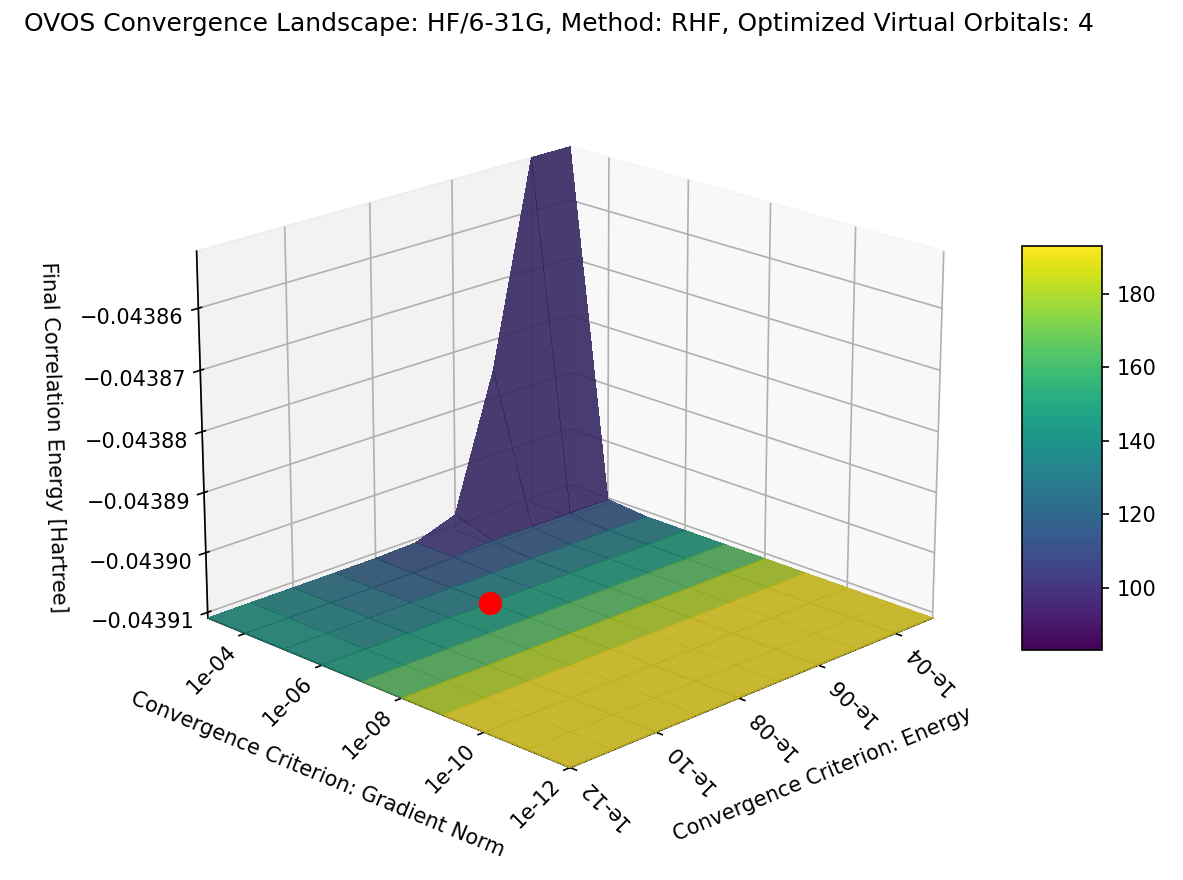
\includegraphics[width=0.9\textwidth]{figures/Ekstra/ovos_convergence_landscape.png}
    \caption{Convergence iteration count landscape for OVOS with convergence criteria gradient norm and MP2 correlation energy. Explored for the HF molecule in the 6--31G basis with initial RHF orbitals. Active space of 7 molecular orbitals. The red point indicates the final converged solution with the default criteria. }
    \label{fig:convergence_landscape}
\end{figure}

The next section describes the different initialisation strategies implemented and their impact on convergence.

\section{Initialisation Strategies}
\label{sec:method_initialisation_strategies}

Here we detail the three distinct initialisation strategies implemented for the OVOS algorithm, which can significantly affect convergence speed and the quality of the final orbital set found by the Newton-Raphson iteration.

\subsection{Default SCF Initialisation}

We can utilise the canonical MO coefficients obtained from a preceding RHF or UHF SCF calculation as the initial guess for the OVOS iteration, like PySCF \code{scf.RHF()}. This is the default strategy and is computationally efficient, as it leverages the existing SCF machinery to provide a reasonable starting point. As seen in Code~\ref{lst:scf_init}, the initial MO coefficients, the SCF object, and the Fock matrices are passed directly to the OVOS constructor, and the iteration proceeds from there. 

\newpage

\begin{lstlisting}[style=python, caption={OVOS initialization with RHF/UHF starting guess}, label=lst:scf_init]
ovos = OVOS(
    mol=mol,
    scf="scf",          
    Fao=[Fao_alpha, Fao_beta], 
    num_opt_virtual_orbs=4,  
    mo_coeff=[mo_a, mo_b],   
    init_orbs="RHF",         
    verbose=1,
    max_iter=1000,
    conv_energy=1e-8,
    conv_grad=1e-4,
    keep_track_max=50
)

# Run from scratch
E_corr, E_hist, iters, mo_final, fock_final, reason = ovos.run(mo_coeff, fock_spin=None)
\end{lstlisting}

If no initial Fock matrix is provided in \code{ovos.run} in Code~\ref{lst:scf_init}, it is constructed from the AO Fock matrices and the initial MO coefficients, as shown in Code~\ref{lst:init_fock}. This ensures that the MP1 amplitudes and MP2 energy can be computed correctly in the first iteration.

\begin{lstlisting}[style=python, caption={Initial Fock matrix construction}, label=lst:init_fock]
if fock_spin is None:
    # Transform AO Fock to MO basis
    Fmo_a = mo_coeffs[0].T @ self.Fao[0] @ mo_coeffs[0]
    Fmo_b = mo_coeffs[1].T @ self.Fao[1] @ mo_coeffs[1]
    
    # Build spin-orbital Fock (block-diagonal alpha/beta)
    fock_spin = self._build_spin_fock(Fmo_a, Fmo_b)
    
    # Extract diagonal energies for MP2 denominators
    eig_a = scipy.linalg.eigh(Fmo_a, eigvals_only=True)
    eig_b = scipy.linalg.eigh(Fmo_b, eigvals_only=True)
    self.eps = self._spatial_to_spin_energies(eig_a, eig_b)
\end{lstlisting}

\subsection{Warm-Start from Previous Orbital Set}

For a systematic scan over different numbers of active virtual orbitals $N'_{\rm virt} = 2, 4, 6, \ldots$, we can adopt a warm-start strategy where the converged orbitals from a previous run with $N'_{\rm virt}=k$ active virtuals are used as the starting guess for the next run with $N'_{\rm virt}=k+2$ active virtuals. The rationale behind this approach is that nearby orbital spaces should have similar optimal MOs, and thus using the previously optimised orbitals can provide a better starting point for convergence, potentially improving the recovery fraction and reducing the iteration count. The pseudo-code for this strategy is shown in Code~\ref{lst:warmstart}, see Appendix~\ref{appc:code} for the full implementation.

\begin{lstlisting}[style=python, caption={Warm-start strategy (pseudo-code for expansion)}, label=lst:warmstart]
# Previous run with N'_{\rm virt}=2 active virtuals
ovos_prev = OVOS(mol, scf, Fao, num_opt_virtual_orbs=2, mo_coeff=..., ...)
E_2, _, _, mo_prev, fock_prev, _ = ovos_prev.run(mo_coeff_scf, fock_spin=None)

# Use optimized orbitals as starting guess for N'_{\rm virt}=4
ovos_curr = OVOS(mol, scf, Fao, num_opt_virtual_orbs=4, 
                 mo_coeff=mo_prev,  # Start from previous optimum
                 ...)
E_4, _, _, mo_curr, fock_curr, _ = ovos_curr.run(mo_prev, fock_spin=fock_prev)
\end{lstlisting}


\subsection{Random Unitary Sampling}

To explore the orbital space landscape more thoroughly and potentially avoid local minima, we implement a random unitary sampling strategy. In this approach, we generate a number of random unitary rotations in the virtual orbital space by creating random matrices and orthogonalizing them using QR decomposition. Each random unitary is applied to the virtual orbital block of the initial MO coefficients, and the OVOS iteration is run from each of these starting points. The result with the lowest MP2 correlation energy $J_2$ at convergence is selected as the final output. This method is computationally expensive, as it requires running the full OVOS iteration \code{n_samples} times. The conceptual code for this strategy is shown in Code~\ref{lst:random_unitary}, see Appendix~\ref{appc:code} for the full implementation.

\begin{lstlisting}[style=python, caption={Random unitary initialization}, label=lst:random_unitary]
# Generate random unitary rotations in virtual space
n_samples = 500
best_energy = np.inf
for sample in range(n_samples):
    # Generate random matrix and orthogonalize via QR
    random_matrix = np.random.randn(nvir, nvir)
    Q, R = np.linalg.qr(random_matrix)
    # Apply to virtual orbital block
    mo_rot = mo_coeff.copy()
    mo_rot[:, nelec:] = mo_coeff[:, nelec:] @ Q
    # Run OVOS from this starting point
    ovos = OVOS(mol, scf, Fao, num_opt_virtual_orbs, mo_rot, ...)
    E, E_hist, _, mo_best, _, _ = ovos.run(mo_rot)
    # Track lowest energy
    if E < best_energy:
        best_energy = E
        mo_best_overall = mo_best
# Use best result across all 500 random starts
return mo_best_overall, best_energy
\end{lstlisting}

